\documentclass{standalone}
\usepackage{tikz}
\usetikzlibrary{patterns, positioning}


\begin{document}
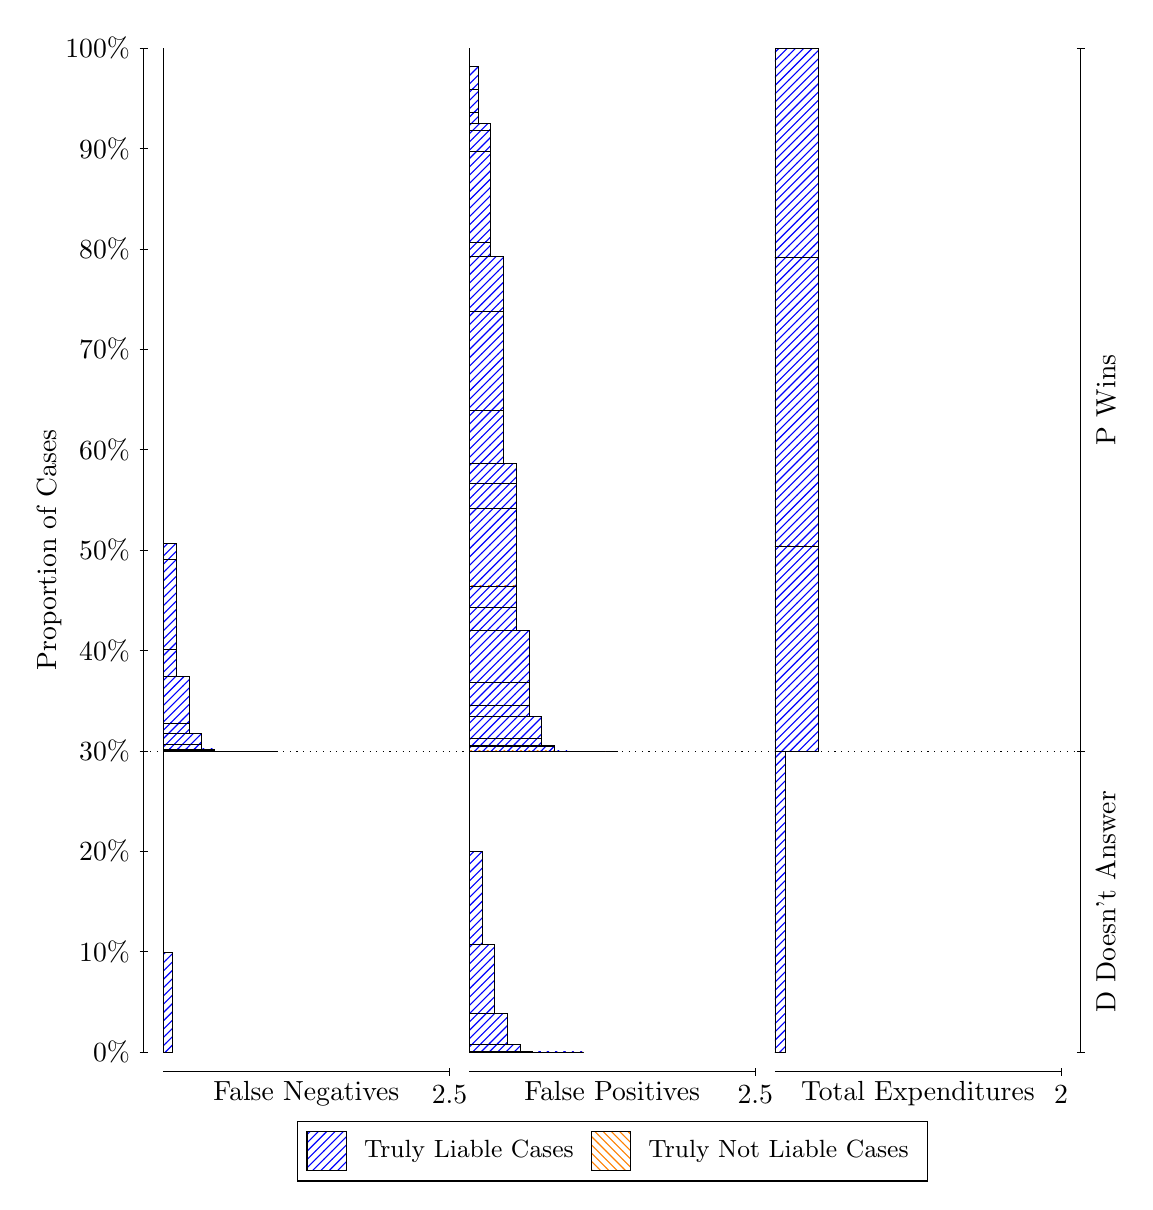
\begin{tikzpicture}
\draw[black, very thin] (1.5,1.75) -- (1.5,14.5);
\node[rotate=90, text=black, anchor=center] at (0.3, 8.125) {Proportion of Cases};
\draw[black, very thin] (1.45,1.75) -- (1.55,1.75);
\node[text=black, anchor=east] at (1.45, 1.75) {0\%};
\draw[black, very thin] (1.45,3.025) -- (1.55,3.025);
\node[text=black, anchor=east] at (1.45, 3.025) {10\%};
\draw[black, very thin] (1.45,4.3) -- (1.55,4.3);
\node[text=black, anchor=east] at (1.45, 4.3) {20\%};
\draw[black, very thin] (1.45,5.575) -- (1.55,5.575);
\node[text=black, anchor=east] at (1.45, 5.575) {30\%};
\draw[black, very thin] (1.45,6.85) -- (1.55,6.85);
\node[text=black, anchor=east] at (1.45, 6.85) {40\%};
\draw[black, very thin] (1.45,8.125) -- (1.55,8.125);
\node[text=black, anchor=east] at (1.45, 8.125) {50\%};
\draw[black, very thin] (1.45,9.4) -- (1.55,9.4);
\node[text=black, anchor=east] at (1.45, 9.4) {60\%};
\draw[black, very thin] (1.45,10.675) -- (1.55,10.675);
\node[text=black, anchor=east] at (1.45, 10.675) {70\%};
\draw[black, very thin] (1.45,11.95) -- (1.55,11.95);
\node[text=black, anchor=east] at (1.45, 11.95) {80\%};
\draw[black, very thin] (1.45,13.225) -- (1.55,13.225);
\node[text=black, anchor=east] at (1.45, 13.225) {90\%};
\draw[black, very thin] (1.45,14.5) -- (1.55,14.5);
\node[text=black, anchor=east] at (1.45, 14.5) {100\%};

\draw[black, very thin] (13.4,1.75) -- (13.4,14.5);
\draw[black, very thin] (13.35,1.75) -- (13.45,1.75);
\node[anchor=west] at (13.35, 1.75) {};
\draw[black, very thin] (13.35,5.5631) -- (13.45,5.5631);
\node[anchor=west] at (13.35, 5.5631) {};
\draw[black, very thin] (13.35,14.5) -- (13.45,14.5);
\node[anchor=west] at (13.35, 14.5) {};

\draw[black, very thin, pattern color=blue, pattern=north east lines] (1.75,1.75) rectangle (1.859,3.0136);
\draw[black, very thin, pattern color=orange, pattern=north west lines] (1.75,3.0136) rectangle (1.75,3.0136);
\draw[black, very thin, pattern color=blue, pattern=north east lines] (1.75,3.0136) rectangle (1.75,5.5631);
\draw[black, very thin, pattern color=blue, pattern=north east lines] (1.75,5.5631) rectangle (3.2033,5.5631);
\draw[black, very thin, pattern color=blue, pattern=north east lines] (1.75,5.5631) rectangle (3.0419,5.5631);
\draw[black, very thin, pattern color=blue, pattern=north east lines] (1.75,5.5631) rectangle (2.8804,5.5631);
\draw[black, very thin, pattern color=blue, pattern=north east lines] (1.75,5.5631) rectangle (2.8804,5.5631);
\draw[black, very thin, pattern color=blue, pattern=north east lines] (1.75,5.5631) rectangle (2.7189,5.5631);
\draw[black, very thin, pattern color=blue, pattern=north east lines] (1.75,5.5631) rectangle (2.7189,5.5632);
\draw[black, very thin, pattern color=blue, pattern=north east lines] (1.75,5.5632) rectangle (2.5574,5.5664);
\draw[black, very thin, pattern color=blue, pattern=north east lines] (1.75,5.5664) rectangle (2.3959,5.5801);
\draw[black, very thin, pattern color=blue, pattern=north east lines] (1.75,5.5801) rectangle (2.3959,5.5994);
\draw[black, very thin, pattern color=blue, pattern=north east lines] (1.75,5.5994) rectangle (2.2344,5.6611);
\draw[black, very thin, pattern color=blue, pattern=north east lines] (1.75,5.6611) rectangle (2.2344,5.792);
\draw[black, very thin, pattern color=blue, pattern=north east lines] (1.75,5.792) rectangle (2.2344,5.7961);
\draw[black, very thin, pattern color=blue, pattern=north east lines] (1.75,5.7961) rectangle (2.073,5.9283);
\draw[black, very thin, pattern color=blue, pattern=north east lines] (1.75,5.9283) rectangle (2.073,6.519);
\draw[black, very thin, pattern color=blue, pattern=north east lines] (1.75,6.519) rectangle (1.9115,6.8616);
\draw[black, very thin, pattern color=blue, pattern=north east lines] (1.75,6.8616) rectangle (1.9115,8.0021);
\draw[black, very thin, pattern color=blue, pattern=north east lines] (1.75,8.0021) rectangle (1.9115,8.2127);
\draw[black, very thin, pattern color=orange, pattern=north west lines] (1.75,8.2127) rectangle (1.75,8.2127);
\draw[black, very thin, pattern color=blue, pattern=north east lines] (1.75,8.2127) rectangle (1.75,14.5);
\draw[black, very thin, pattern color=orange, pattern=north west lines] (5.6333,1.75) rectangle (7.0867,1.75);
\draw[black, very thin, pattern color=blue, pattern=north east lines] (5.6333,1.75) rectangle (7.0867,1.75);
\draw[black, very thin, pattern color=blue, pattern=north east lines] (5.6333,1.75) rectangle (6.9252,1.75);
\draw[black, very thin, pattern color=blue, pattern=north east lines] (5.6333,1.75) rectangle (6.7637,1.75);
\draw[black, very thin, pattern color=blue, pattern=north east lines] (5.6333,1.75) rectangle (6.6022,1.7503);
\draw[black, very thin, pattern color=blue, pattern=north east lines] (5.6333,1.7503) rectangle (6.4407,1.7582);
\draw[black, very thin, pattern color=blue, pattern=north east lines] (5.6333,1.7582) rectangle (6.2793,1.8434);
\draw[black, very thin, pattern color=blue, pattern=north east lines] (5.6333,1.8434) rectangle (6.1178,2.2366);
\draw[black, very thin, pattern color=blue, pattern=north east lines] (5.6333,2.2366) rectangle (5.9563,3.1157);
\draw[black, very thin, pattern color=blue, pattern=north east lines] (5.6333,3.1157) rectangle (5.7948,4.2995);
\draw[black, very thin, pattern color=blue, pattern=north east lines] (5.6333,4.2995) rectangle (5.6333,5.5631);
\draw[black, very thin, pattern color=orange, pattern=north west lines] (5.6333,5.5631) rectangle (7.5227,5.5631);
\draw[black, very thin, pattern color=blue, pattern=north east lines] (5.6333,5.5631) rectangle (7.5227,5.5631);
\draw[black, very thin, pattern color=orange, pattern=north west lines] (5.6333,5.5631) rectangle (7.3612,5.5631);
\draw[black, very thin, pattern color=blue, pattern=north east lines] (5.6333,5.5631) rectangle (7.3612,5.5631);
\draw[black, very thin, pattern color=blue, pattern=north east lines] (5.6333,5.5631) rectangle (7.1997,5.5631);
\draw[black, very thin, pattern color=orange, pattern=north west lines] (5.6333,5.5631) rectangle (7.1997,5.5631);
\draw[black, very thin, pattern color=blue, pattern=north east lines] (5.6333,5.5631) rectangle (7.1997,5.5631);
\draw[black, very thin, pattern color=blue, pattern=north east lines] (5.6333,5.5631) rectangle (7.0382,5.5632);
\draw[black, very thin, pattern color=blue, pattern=north east lines] (5.6333,5.5632) rectangle (7.0382,5.5634);
\draw[black, very thin, pattern color=orange, pattern=north west lines] (5.6333,5.5634) rectangle (7.0382,5.5634);
\draw[black, very thin, pattern color=blue, pattern=north east lines] (5.6333,5.5634) rectangle (7.0382,5.5638);
\draw[black, very thin, pattern color=orange, pattern=north west lines] (5.6333,5.5638) rectangle (6.8767,5.5638);
\draw[black, very thin, pattern color=blue, pattern=north east lines] (5.6333,5.5638) rectangle (6.8767,5.5694);
\draw[black, very thin, pattern color=blue, pattern=north east lines] (5.6333,5.5694) rectangle (6.8767,5.5711);
\draw[black, very thin, pattern color=blue, pattern=north east lines] (5.6333,5.5711) rectangle (6.8767,5.5729);
\draw[black, very thin, pattern color=orange, pattern=north west lines] (5.6333,5.5729) rectangle (6.7153,5.5729);
\draw[black, very thin, pattern color=blue, pattern=north east lines] (5.6333,5.5729) rectangle (6.7153,5.6346);
\draw[black, very thin, pattern color=blue, pattern=north east lines] (5.6333,5.6346) rectangle (6.7153,5.6459);
\draw[black, very thin, pattern color=blue, pattern=north east lines] (5.6333,5.6459) rectangle (6.5538,5.7306);
\draw[black, very thin, pattern color=orange, pattern=north west lines] (5.6333,5.7306) rectangle (6.5538,5.7306);
\draw[black, very thin, pattern color=blue, pattern=north east lines] (5.6333,5.7306) rectangle (6.5538,6.0073);
\draw[black, very thin, pattern color=blue, pattern=north east lines] (5.6333,6.0073) rectangle (6.3923,6.15);
\draw[black, very thin, pattern color=blue, pattern=north east lines] (5.6333,6.15) rectangle (6.3923,6.4432);
\draw[black, very thin, pattern color=orange, pattern=north west lines] (5.6333,6.4432) rectangle (6.3923,6.4432);
\draw[black, very thin, pattern color=blue, pattern=north east lines] (5.6333,6.4432) rectangle (6.3923,7.1082);
\draw[black, very thin, pattern color=blue, pattern=north east lines] (5.6333,7.1082) rectangle (6.2308,7.3986);
\draw[black, very thin, pattern color=blue, pattern=north east lines] (5.6333,7.3986) rectangle (6.2308,7.6699);
\draw[black, very thin, pattern color=orange, pattern=north west lines] (5.6333,7.6699) rectangle (6.2308,7.6699);
\draw[black, very thin, pattern color=blue, pattern=north east lines] (5.6333,7.6699) rectangle (6.2308,8.6537);
\draw[black, very thin, pattern color=blue, pattern=north east lines] (5.6333,8.6537) rectangle (6.2308,8.9731);
\draw[black, very thin, pattern color=blue, pattern=north east lines] (5.6333,8.9731) rectangle (6.2308,9.2243);
\draw[black, very thin, pattern color=blue, pattern=north east lines] (5.6333,9.2243) rectangle (6.0693,9.8998);
\draw[black, very thin, pattern color=orange, pattern=north west lines] (5.6333,9.8998) rectangle (6.0693,9.8998);
\draw[black, very thin, pattern color=blue, pattern=north east lines] (5.6333,9.8998) rectangle (6.0693,11.16);
\draw[black, very thin, pattern color=blue, pattern=north east lines] (5.6333,11.16) rectangle (6.0693,11.85);
\draw[black, very thin, pattern color=blue, pattern=north east lines] (5.6333,11.85) rectangle (5.9079,12.038);
\draw[black, very thin, pattern color=blue, pattern=north east lines] (5.6333,12.038) rectangle (5.9079,13.185);
\draw[black, very thin, pattern color=blue, pattern=north east lines] (5.6333,13.185) rectangle (5.9079,13.456);
\draw[black, very thin, pattern color=blue, pattern=north east lines] (5.6333,13.456) rectangle (5.9079,13.544);
\draw[black, very thin, pattern color=blue, pattern=north east lines] (5.6333,13.544) rectangle (5.7464,13.689);
\draw[black, very thin, pattern color=blue, pattern=north east lines] (5.6333,13.689) rectangle (5.7464,13.98);
\draw[black, very thin, pattern color=blue, pattern=north east lines] (5.6333,13.98) rectangle (5.7464,14.267);
\draw[black, very thin, pattern color=blue, pattern=north east lines] (5.6333,14.267) rectangle (5.6333,14.5);
\draw[black, very thin, pattern color=orange, pattern=north west lines] (9.5167,1.75) rectangle (9.6529,1.75);
\draw[black, very thin, pattern color=blue, pattern=north east lines] (9.5167,1.75) rectangle (9.6529,5.5631);
\draw[black, very thin, pattern color=orange, pattern=north west lines] (9.5167,5.5631) rectangle (10.062,5.5631);
\draw[black, very thin, pattern color=blue, pattern=north east lines] (9.5167,5.5631) rectangle (10.062,8.1766);
\draw[black, very thin, pattern color=orange, pattern=north west lines] (9.5167,8.1766) rectangle (10.062,8.1766);
\draw[black, very thin, pattern color=blue, pattern=north east lines] (9.5167,8.1766) rectangle (10.062,11.84);
\draw[black, very thin, pattern color=orange, pattern=north west lines] (9.5167,11.84) rectangle (10.062,11.84);
\draw[black, very thin, pattern color=blue, pattern=north east lines] (9.5167,11.84) rectangle (10.062,14.5);
\draw[black, dotted] (1.5,5.5631) -- (13.4,5.5631);
\draw[black, very thin] (1.75,1.5) -- (5.3833,1.5);
\node[text=black, anchor=north] at (3.5667, 1.5) {False Negatives};
\draw[black, very thin] (5.3833,1.45) -- (5.3833,1.55);
\node[text=black, anchor=north] at (5.3833, 1.45) {2.5};

\draw[black, very thin] (5.6333,1.5) -- (9.2667,1.5);
\node[text=black, anchor=north] at (7.45, 1.5) {False Positives};
\draw[black, very thin] (9.2667,1.45) -- (9.2667,1.55);
\node[text=black, anchor=north] at (9.2667, 1.45) {2.5};

\draw[black, very thin] (9.5167,1.5) -- (13.15,1.5);
\node[text=black, anchor=north] at (11.333, 1.5) {Total Expenditures};
\draw[black, very thin] (13.15,1.45) -- (13.15,1.55);
\node[text=black, anchor=north] at (13.15, 1.45) {2};

\node[text=black, centered, rotate=90] at (13.72, 3.6565) {D Doesn't Answer};
\node[text=black, centered, rotate=90] at (13.72, 10.032) {P Wins};

\draw (7.449999999999999,1.5) node[draw=none] (baseCoordinate) {};
\begin{scope}[align=center]
        \matrix[scale=0.5, draw=black, below=0.5cm of baseCoordinate, nodes={draw}, column sep=0.1cm]{
            \node[rectangle, draw, minimum width=0.5cm, minimum height=0.5cm, pattern color=blue, pattern=north east lines] {}; &
            \node[draw=none, font=\small, text=black] (B) {Truly Liable Cases}; &
            \node[rectangle, draw, minimum width=0.5cm, minimum height=0.5cm, pattern color=orange, pattern=north west lines] {}; &
            \node[draw=none, font=\small, text=black] (B) {Truly Not Liable Cases}; \\
            };
\end{scope}

\end{tikzpicture}
\end{document}